\documentclass{beamer}
\usepackage[utf8]{inputenc}
\usepackage{subfiles}
\usepackage{lipsum}
\usepackage{float}
\usepackage{listings}
\usepackage{color}
\usepackage{tikz}
\usepackage{lmodern}

\definecolor{darkblue}{rgb}{0.086,0.145,0.357}
\definecolor{darkpurple}{rgb}{0.3098,0 , 0.3098}
\definecolor{skinorange}{rgb}{0.957,0.639 , 0.365}


\usetikzlibrary{arrows.meta,arrows}
\usetikzlibrary{positioning}

\usetheme{Madrid}
\usecolortheme{beaver}

\title[About Beamer]{Priority Queue}
\subtitle{An Introduction}

\author[A.A. and A.N.F]{Md Awsaf Alam \inst{1} \\ Ahmed Nafis Fuad\inst{2}}

\institute{
\inst{1}
Department of CSE\\
BUET\\
\inst{2}
Department of CSE\\
BUET
}

\date{\today}

\AtBeginSection[]{
\begin{frame}
    \tableofcontents[currentsection]
\end{frame}
}

\begin{document}
\titlepage

\begin{frame}{Table of Contents}
\tableofcontents

\end{frame}
\section{What is a Priority Queue?}

\begin{frame}
\frametitle{What is a Priority Queue?}

A priority queue is an abstract data type which is like a regular queue or stack data structure,
but where additionally each element has a "priority" associated with it.
 In a priority queue, an element with high priority is served before an element with low priority.

A Binary (Max) Heap is a complete binary tree that maintains the Max Heap property.
Binary Heap is one possible data structure to model an efficient Priority Queue (PQ) Abstract Data Type (ADT). In a PQ, each element has a "priority" and an element with higher priority is served before an element with lower priority (ties are broken with standard First-In First-Out (FIFO) rule as with normal Queue). Try clicking ExtractMax() for a sample animation on extracting the max value of random Binary Heap above.
To focus the discussion scope, we design this visualization to show a Binary Max Heap that contains distinct integers only.

\end{frame}
\begin{frame}
\frametitle{What is a Queue?}
\begin{columns}
  \column{0.2\textwidth}

A queue is an example of a linear data structure, or more abstractly a sequential collection.
Queues provide services in computer science, transport,
and operations research where various entities such as data, objects,
persons, or events are stored and held to be processed later.
  \column{0.7\textwidth}


  \tikzset{every picture/.style={line width=0.15pt}} %set default line width to 0.75pt

  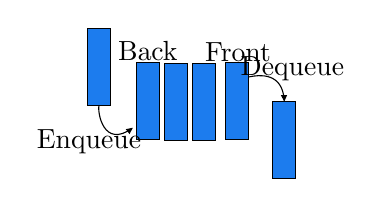
\begin{tikzpicture}[x=0.75pt,y=0.75pt,yscale=-0.35,xscale=0.35]
  %uncomment if require: \path (0,300); %set diagram left start at 0, and has height of 300

  \draw  [fill={rgb, 255:red, 28; green, 124; blue, 238 }  ,fill opacity=1 ]  (100, 62.67) rectangle (131.67, 169)   ;
  \draw  [fill={rgb, 255:red, 28; green, 124; blue, 238 }  ,fill opacity=1 ]  (138, 63.67) rectangle (169.67, 170)   ;
  \draw  [fill={rgb, 255:red, 28; green, 124; blue, 238 }  ,fill opacity=1 ]  (222, 62.67) rectangle (253.67, 169)   ;
  \draw  [fill={rgb, 255:red, 28; green, 124; blue, 238 }  ,fill opacity=1 ]  (177, 63.67) rectangle (208.67, 170)   ;
  \draw  [fill={rgb, 255:red, 28; green, 124; blue, 238 }  ,fill opacity=1 ]  (287, 116.67) rectangle (318.67, 223)   ;
  \draw  [fill={rgb, 255:red, 28; green, 124; blue, 238 }  ,fill opacity=1 ]  (32, 15.67) rectangle (63.67, 122)   ;
  \draw    (47.83,122) .. controls (45.36,131.57) and (54.15,181.65) .. (93.14,153.54) ;
  \draw [shift={(94.33,152.67)}, rotate = 503.13] [fill={rgb, 255:red, 0; green, 0; blue, 0 }  ][line width=0.75]  [draw opacity=0] (8.93,-4.29) -- (0,0) -- (8.93,4.29) -- cycle    ;

  \draw    (254.33,82.67) .. controls (268.12,79.71) and (300.35,75.79) .. (302.74,114.85) ;
  \draw [shift={(302.83,116.67)}, rotate = 267.9] [fill={rgb, 255:red, 0; green, 0; blue, 0 }  ][line width=0.75]  [draw opacity=0] (8.93,-4.29) -- (0,0) -- (8.93,4.29) -- cycle    ;


  \draw (34,172) node  [align=left] {Enqueue};
  \draw (314,72) node  [align=left] {Dequeue};
  \draw (115,47) node  [align=left] {Back};
  \draw (239,49) node  [align=left] {Front};


  \end{tikzpicture}

\end{columns}

\end{frame}

\begin{frame}
\frametitle{What is a  Queue?}

\begin{columns}
  \column{0.1\textwidth}

  \column{0.1\textwidth}
    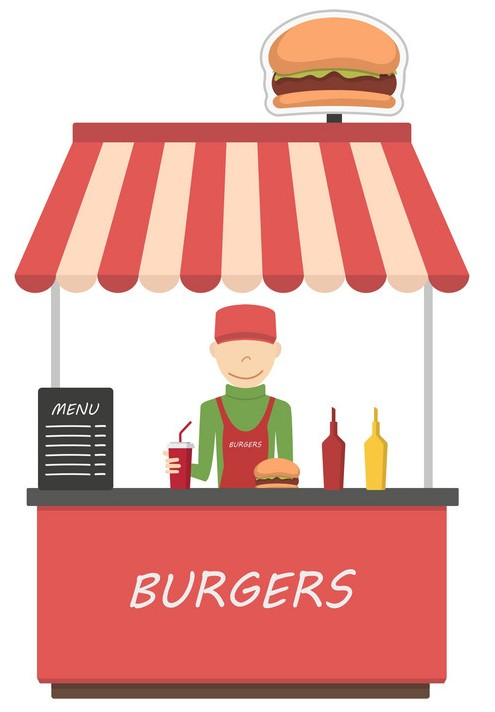
\includegraphics[height=1.6cm]{Image/Burger_Stall.jpg} \pause
  \column{0.1\textwidth}
      
\includegraphics[height=1.6cm]{Image/pikachu.jpg}
  \begin{center}
    $1$ \pause
  \end{center}

  \column{0.1\textwidth}
    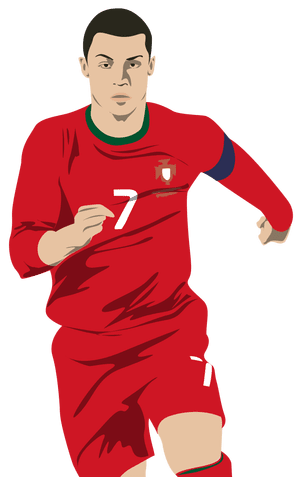
\includegraphics[height=1.6cm]{Image/ronaldo.png}
    \begin{center}
      $1$ \pause
    \end{center}
  \column{0.1\textwidth}
    
\includegraphics[height=1.6cm]{Image/trump.jpg}
    \begin{center}
      $1$ \pause
    \end{center}

  \column{0.1\textwidth}
    
\includegraphics[height=1.6cm]{Image/putin.jpg}
    \begin{center}
      $1$ \pause
    \end{center}

  \end{columns}

\end{frame}


\section{Problem Definition}
\begin{frame}{Simulation}

\end{frame}


\begin{frame}{Another Simulation}
\setbeamercovered{dynamic}
\begin{center}
  \begin{tabular}{|c|c|c|}
      \hline
      Table & X & Y\\
      \hline
      A & \onslide<1->{1} & \onslide<2->{0}  \\
      \hline
      B & \onslide<3->{0} & \onslide<4->{1}  \\
      \hline
  \end{tabular}
\end{center}

\end{frame}


\section{Motivation}

\begin{frame}{Use of Columns and Images}
\setbeamercovered{dynamic}  % Ghola korar jonno

  \begin{columns}
    \column{0.5\textwidth}

    \begin{figure}[H]
        \centering
        \label{fig:2}
        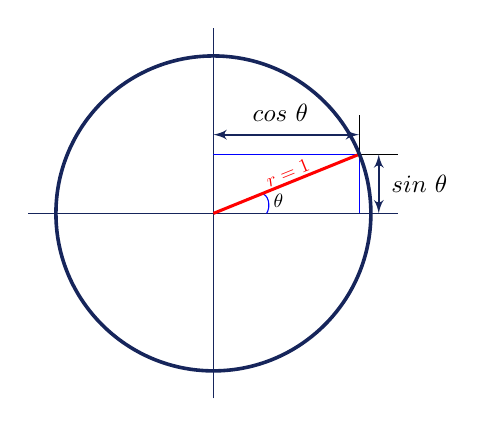
\begin{tikzpicture}[scale=0.5]

           \draw [darkblue,line width= 0.5pt] (-4.7,0) -- (4.7,0);
           \draw [darkblue,line width= 0.5pt] (0,-4.7) -- (0,4.7);

           \draw [blue] (0,1.5) -- (3.7,1.5);
           \draw [darkblue,line width= 0.7pt,{latex'[width= 5pt, length=5pt]}-{latex'[width= 5mm, length=5mm]}] (0,2) -- (3.7,2);
           \node [scale = 0.9pt, above] at (1.7 , 2.1){$cos ~\theta$};

           \draw (3.7,1.5) -- (4.7,1.5);

           \draw [blue] (3.7,0) -- (3.7,1.5);
           \draw [darkblue,line width= 0.7pt,{latex'[width= 5pt, length=5pt]}-{latex'[width= 5mm, length=5mm]}] (4.2,0) -- (4.2,1.5);
           \node [scale = 0.9pt, right] at (4.3, 0.75){$sin ~\theta$};

           \draw (3.7,1.5) -- (3.7,2.5);

           \draw [blue](1.35 , 0) to [in=5,out=55] (1.2, 0.50);
           \node [scale = 0.7pt ,above] at (1.65, -0.02){$\theta$};

           \draw [red,line width= 1.1pt] (0,0) -- (3.7,1.5);
          \node [scale = 0.7pt,red,rotate = 22 ,right] at (1.2, 0.75){$r = 1$};

          \draw[darkblue,line width= 1.3pt] (0,0) circle (4);

        \end{tikzpicture}

        \caption{Alternate representation of Pythagorean theorem.}
    \end{figure}

    \column{0.5\textwidth}

    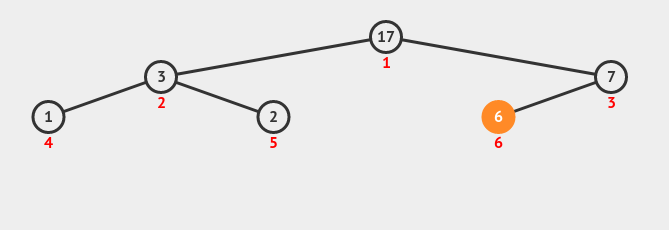
\includegraphics[height=1.6cm]{Image/tree.png}
    \end{columns}

\end{frame}

\section{Design}

\section{Previous Works}
\begin{frame}{Blocks}
    \begin{block}{Sample Block}
    This is a sample block.
    \end{block}
    \begin{alertblock}{Sample Alert Block}
    This is a sample \textbf<2>{alert block}.
    \end{alertblock}
    \begin{example}
    Sample \textcolor<3->{red}{example}.
    \end{example}
\end{frame}
\section{Conclusion}
\subfile{sec/tree_animation.tex}


\end{document}
\begin{frame}{Use of Columns and Images}
    COncluded
\end{frame}
